\documentclass[letterpaper,12pt]{article}
\usepackage[utf8]{inputenc}
\usepackage[T1]{fontenc}
\usepackage[spanish]{babel}
\usepackage{amsmath,amssymb}
\usepackage{url}
\usepackage{graphicx}
\usepackage[left=2.54cm,right=2.54cm,top=2.54cm,bottom=2.54cm]{geometry}
\setlength{\parskip}{0.8em}
\setlength{\parindent}{0pt}
\setlength{\emergencystretch}{2em}
\pagestyle{plain}

\begin{document}
\begingroup
\sloppy
\ttfamily
\obeylines
\catcode`\^^M=5\relax
\newcommand{\bigtitle}[1]{\par\begin{center}\normalfont\Huge\bfseries #1\end{center}\par}
\newcommand{\medtitle}[1]{\par\begin{center}\normalfont\Large\bfseries #1\end{center}\par}
\newcommand{\smalltitle}[1]{{\par\noindent\normalfont\large\bfseries #1\par}}
(portada)
\newpage

                   ÍNDICE

1. Introducción y justificación
2. Desarrollo y fundamento Matemático
3. Aplicación Práctica
4. Conclusiones
5. Referencias






\newpage
\bigtitle{1. Introducción y justificación}
La tecnología Bluetooth es uno de los estándares de comunicación inalámbrica a corta distancia
más extendidos en el campo de la informática actual. Sus usos van desde conectarse a periféricos
sencillos (como auriculares, teclados...) hasta comunicaciones más complejas, como vehículos,
dispositivos médicos, o tecnologías IoT (Internet Of Things).

El funcionamiento del Bluetooth no se limita a transmitir señales de radio. Detrás de esta
tecnología se encuentran variedad de algoritmos y procesos matemáticos que aseguran la fiabilidad,
eficiencia y seguridad de la información transmitida. Aquí entran en juego el uso de vectores,
matrices y transformaciones lineales en distintos niveles del sistema, como la codificación de
señales o los protocolos criptográficos.

El Bluetooth basa su funcionamiento en la transmisión de señales mediante RF en la banda de
2.4GHz, usando una técnica conocida como "frequency hopping spread spectrum" (FHSS). Esta
técnica consiste en cambiar rápidamente la frecuencia de transmisión siguiendo una secuencia
pseudoaleatoria, lo que reduce interferencias y mejora la seguridad contra escuchas externas. Este
proceso se puede modelar matemáticamente mediante estructuras vectoriales y matrices de
transformación, ya que las señales pueden ser representadas como vectores en espacios n-
dimensionales que serán transformados mediante distintas operaciones lineales durante los
procesos de modulación, transmisión y decodificación.

La codificación y corrección de errores también están basadas en álgebra lineal. En un entorno
inalámbrico, las señales se pueden ver afectadas por ruido, interferencias o pérdidas de
información. Para evitar y solventar estos problemas, se aplican operaciones a los vectores de datos
dentro de espacios vectoriales. Estas operaciones introducen redundancia controlada en los datos,
de tal manera que el receptor puede aplicar operaciones matriciales de verificación para comprobar
la información.






\newpage
También encontraremos elementos de álgebra lineal en la representación y procesamiento de
señales digitales. Las señales transmitidas se pueden describir como vectores en espacios de
funciones discretas, y las operaciones de procesamiento (filtrado, compresión, detección...) pueden
representarse como transformaciones lineales.




La importancia del Bluetooth en la informática se explica por varios factores. En primer lugar, su
presencia en todos los dispositivos del día a día: toda la tecnología que usamos habitualmente tiene
soporte para Bluetooth (portátiles, teléfonos, auriculares, smart-watches...)

También desempeña un papel importantísimo en el desarrollo del IoT. La versión BLE (Bluetooth
Low Energy) está diseñada específicamente para dispositivos de bajo consumo, como sensores, o
sistemas de autorización. En estos contextos donde la capacidad de establecer redes de dispositivos
que intercambian información, la eficiencia es crucial.

La seguridad también se ha vuelto un aspecto crítico, ya que se usa esta tecnología para
dispositivos que intercambian datos personales (auriculares con acceso a asistentes de IA,
dispositivos médicos...). Los mecanismos criptográficos/matemáticos implementados en el
Bluetooth buscan garantizar la confidencialidad, integridad y disponibilidad (tríada CIA) de los
datos.

El Bluetooth nos parece un buen ejemplo de cómo los conceptos matemáticos que de primeras
parecen abstractos, tienen aplicaciones prácticas en tecnologías de las que dependemos y usamos
diariamente.





\newpage
\bigtitle{2. Desarrollo y fundamento Matemático}
Aunque la implementación física del Bluetooth se base en radiofrecuencia y protocolos de
comunicación complejos, la información que viaja entre dispositivos se representa como
estructuras matemáticas discretas. Esta abstracción permite modelar señales y errores como
vectores y espacios vectoriales.

\medtitle{2.1 Modelización vectorial de las señales digitales}
\smalltitle{2.1.1 Representación de información digital como vectores}
Definimos vector como un elemento de un espacio vectorial. Formalmente, es una tupla ordenada
de elementos pertenecientes a un cuerpo/campo. En contextos de informática, usamos
fundamentalmente dos espacios vectoriales:

$\mathbb{R}^n$ : El espacio de vectores reales de dimensión $n$.

$\mathbb{F}_2^n$ : El espacio de vectores binarios de dimensión $n$, donde el campo $\mathbb{F}_2 = \{0,1\}$ utiliza aritmética
módulo $2$.

En los sistemas de comunicación digital los datos se transmiten como secuencias binarias. Cada
paquete de información puede representarse como un vector binario:

\centerline{$v=(b_1,b_2,b_3,\ldots,b_n),\; b_i\in\{0,1\}$}

Cada componente del vector corresponde a un bit del paquete transmitido. Esta representación
permite aplicar operaciones algebraicas como sumas vectoriales mod. 2 o transformaciones
lineales, que son muy importantes en procesos como la codificación de errores.

En el Bluetooth, los paquetes contienen campos estructurados (cabeceras, direcciones, datos,
códigos de verificación). Cada uno de estos bloques puede ser interpretado como vector.





\newpage
\smalltitle{2.1.2 Espacios vectoriales asociados a la transmisión de datos}
Además de representar directamente los bits, las señales transmitidas también pueden modelarse
como vectores en espacios de dimensión mayor. Cuando un dispositivo Bluetooth transmite
información, la señal se modula y se envía como una secuencia temporal de muestras.

Si se toman n muestras discretas de una señal durante un intervalo de transmisión, estas pueden
representarse como un vector en el espacio:

\centerline{$s=(s_1,s_2,s_3,\ldots,s_n)\in\mathbb{R}^n$}

Cada componente $s_i$ representa la amplitud o fase de la señal en un instante concreto. De esta
forma, el conjunto de todas las posibles señales transmitidas puede interpretarse como un espacio
vectorial de señales.

El proceso de transmisión se puede conceptualizar como:

\centerline{$\text{vector de bits}\to\text{transformación lineal}\to\text{vector de señal}$}

\smalltitle{2.1.3 Interpretación geométrica de la señal transmitida}
Una de las ventajas de representar señales como vectores es la posibilidad de analizar su
comportamiento desde un punto de vista geométrico. En un espacio vectorial, dos vectores se
pueden comparar con una función de distancia. En este contexto, la métrica más relevante es la
distancia de Hamming, que es el número de posiciones en las que difieren dos vectores binarios.

Por ejemplo, $(1,0,1,1)$ y $(1,1,1,0)$ tienen distancia de Hamming $d_H=2$.

Esta medida es esencial para detectar y corregir errores de transmisión. Durante la comunicación,
el ruido/interferencias pueden alterar algunos bits del vector transmitido. Si el sistema tiene
códigos de corrección, puede comparar el vector recibido con los válidos, y elegir el más cercano
según esta métrica.

En el caso de $\mathbb{R}^n$, se usa la distancia euclídea, que mide la distancia geométrica.






\newpage
\medtitle{2.2 Uso de matrices en la codificación y transformación de señales}
\smalltitle{2.2.1 Representación matricial de transformaciones lineales}
Una matriz es una estructura rectangular de elementos pertenecientes a un cuerpo o campo.
Formalmente, una matriz se define como: $A\in\mathbb{R}^{m\times n}$.

Una transformación lineal entre espacios vectoriales puede representarse mediante una matriz.
Siendo $A$ una matriz $m\times n$, la transformación de un vector de datos se expresa como $y = Ax$,
donde '$x$' es el vector de datos original, '$A$' es la matriz de transformación, e '$y$' es el vector
obtenido mediante la combinación lineal de elementos de $x$. Este tipo de operación se usa en
etapas como filtros digitales, transformaciones de bases o procesos de codificación

\smalltitle{2.2.2 Matrices en los procesos de modulación y demodulación}
Uno de los pasos clave en la transmisión de datos es convertirlos en señales físicas que puedan
transmitirse a través del aire. Este proceso se conoce como modulación. Bluetooth usa GFSK
(Gaussian Frequency Shift Keying), y variantes más avanzadas en BLE. Aunque la
implementación real usa procesamiento digital, se puede modelizar mediante transformaciones
lineales.

                                             \centerline{$s = Mx$}

Donde:

$x$ es el vector de datos binarios,

$M$ es una matriz que representa el sistema de modulación,

$s$ es el vector de parámetros de la señal transmitida

En el receptor ocurre el proceso inverso, llamado demodulación. Los algoritmos de demodulación
pueden expresarse mediante sistemas matriciales o problemas de estimación lineal. Habiendo
ruido, el sistema recibido puede modelizarse como:

\centerline{$r=Ax+n$}

Donde $n$ representa el ruido del canal de transmisión. El objetivo del receptor es estimar el vector
'$x$' original a partir del recibido '$r$' (el vector '$y$' del apartado anterior). Esto implica resolver
sistemas lineales o aplicar métodos de optimización.





\newpage
\smalltitle{2.2.3 Matrices generadoras en códigos de corrección de errores.}
Durante la transmisión inalámbrica se producen errores. Para corregirlos se implementan códigos
de corrección, que permiten detectarlos, y a veces revertirlos. Muchos de estos códigos son lineales,
que se describen mediante matrices. En este contexto, el proceso de codificación se realiza
utilizando una matriz generadora $G$. El objetivo es transformar el vector binario en una palabra
codificada:

\centerline{$c=Gm$}

Donde:

$m$ es el vector de información,

$G$ es la matriz generadora,

$C$ es el vector codificado que se transmitirá

La matriz generadora introduce redundancia controlada en el mensaje. Esto significa que se añaden
bits adicionales que no añaden nada nuevo, pero permiten detectar inconsistencias. Este
mecanismo es esencial en el Bluetooth porque el canal radioeléctrico es especialmente vulnerable
a interferencias.

\smalltitle{2.2.4 Matrices de control de paridad}
Además de la matriz G, los códigos utilizan una matriz de control, $H$. Si '$c$' es una palabra válida
   generada por el código, debe cumplir $Hc=0$, donde el vector 0 indica que no hay
                                        inconsistencias.

Cuando el receptor Bluetooth recibe un vector '$r$', calcula $Hr$. Si el resultado es distinto de 0, se
denomina síndrome del error, y proporciona información sobre la posición del posible error en el
vector recibido. En algunos códigos, hasta permite corregir automáticamente el bit incorrecto.

Este proceso puede interpretarse como comprobar si el vector recibido pertenece al subespacio
vectorial generado por las palabras válidas del código. Si no pertenece, necesariamente se ha
producido una alteración.





\newpage
\medtitle{2.3 Subespacios vectoriales en la transmisión y detección de señales}
\smalltitle{2.3.1 Definición formal de subespacio}

Un subespacio vectorial es un subconjunto de un espacio vectorial que cumple las propiedades
necesarias para ser considerado también un espacio. Si V es un espacio vectorial sobre un cuerpo
$F$, un subconjunto $W\subseteq V$ es subespacio si cumple:

   1. El vector nulo pertenece a $W$\\
   2. Si $u,v\in W$, entonces $u+v\in W$\\
   3. Si $u\in W$ y $a\in F$, entonces $au\in W$

Dentro del espacio general $\mathbb{F}_2^n$, ciertas combinaciones de bits corresponden a señales válidas,
mientras que otras no aparecen en la transmisión real. Estas colecciones estructuradas de señales
forman subespacios que representan los códigos usados por el sistema de comunicación.

\smalltitle{2.3.2 Subespacios de códigos válidos}
Como se ha hablado en el apartado 2.2.3, se aplican códigos de corrección de errores que añaden
redundancia a los datos originales. El conjunto de todos los mensajes codificados puede
interpretarse como un subespacio vectorial de todas las posibles cadenas de bits. La '$y$' del
apartado anteriormente mencionado pertenecería necesariamente al subespacio de códigos válidos.
Esto facilita la detección de errores, ya que cualquier vector que no pertenezca al subespacio indica
directamente la presencia de interferencias o corrupción de datos.

\smalltitle{2.3.3 Proyecciones en subespacios para detección de señal}
Durante la transmisión inalámbrica, las señales se ven afectadas por ruido electromagnético,
interferencias de otros dispositivos, y distorsiones del canal. Como resultado, el receptor no acaba
obteniendo exactamente el vector transmitido, sino una versión perturbada.

Si el conjunto de señales válidas se modela como un subespacio $W$ del espacio vectorial de las
señales, la señal recibida se puede interpretar como un vector $r$ que no necesariamente pertenece a
$W$. Para recuperar el mensaje, el sistema de recepción busca el vector de $W$ más cercano a $r$.

Esto equivale a calcular la proyección ortogonal de $r$ sobre $W$. Este procedimiento minimiza la
distancia entre $r$ y una señal válida, eliminando en gran medida la componente del ruido.





\newpage
\smalltitle{2.3.4 Dimensión del subespacio y capacidad del canal}
La dimensión del subespacio de códigos válidos tiene una interpretación directa en este contexto.
Si el subespacio tiene dimensión $k$, estará generado por $k$ vectores linealmente independientes y
\centerline{puede representar $2^k$ mensajes distintos (en el caso binario, claro).}

Sin embargo, los mensajes transmitidos suelen representarse mediante vectores de dimensión $n$,
tal que $n>k$. La diferencia entre $n$ y $k$ representa la redundancia introducida de manera intencionada.

Entonces, mayor dimensión de $k$ implica mayor cantidad de información transmitida, pero menor
diferencia entre $n$ y $k$ implica menor capacidad para detectar errores. Es esencial encontrar un
equilibrio entre ambos factores para mantener el canal eficiente y ser capaces de corregir errores.

\medtitle{2.4 Modelización del canal de transmisión mediante matrices}
\smalltitle{2.4.1 Representación del canal como transformación lineal}
El proceso de transmisión de señal se describe mediante la ecuación

\centerline{$y=Hx+n$}

Siendo:

$H$ la matriz del canal, que representa cómo el medio de transmisión transforma la señal

$x$ es el vector transmitido, con la información ya codificada

$y$ es el vector recibido

$n$ es el vector de ruido añadido durante la transmisión

En la banda de las ondas de radio 2.4GHz, el entorno provoca desvanecimientos, interferencias o
multitrayectoria, fenómenos que se modelan dentro de $H$. Cada elemento de $H$ describe cómo una
componente de la señal afecta a cada componente de la señal recibida. En general, captura las
características del canal inalámbrico en un instante determinado





\newpage
\smalltitle{2.4.2 Interpretación del ruido como perturbación vectorial}
Además de la transformación producida por el canal ($H$), está el ruido ($n$), que se añade al producto
de $Hx$. Por eso, aun conociendo perfectamente el canal $H$, $y$ nunca coincidiría exactamente con
$Hx$. Se asume que el ruido es un vector aleatorio que sigue una distribución normal, lo que se
conoce como ruido gaussiano aditivo o White Gaussian Noise (AWGN).

El AWGN está formado por tres propiedades fundamentales:

   1. Additive (Aditivo)
      Que el ruido sea aditivo significa que se suma directamente a la señal transmitida. Eso
      significa que $y-Hx=n$ \\
   2. Gaussian (Gaussiano)
      El ruido se denomina gaussiano porque cada componente de $n$ sigue una distribución
      normal. Esto nos aporta dos propiedades estadísticas importantes: $\mathbb{E}[n]=0$ y $\mathbb{E}[nn^T]=\sigma^2I$.
      Esto implica que las componentes del ruido son linealmente independientes, y que la
      varianza es la misma en todas las direcciones del espacio vectorial. \\
   3. White (Blanco)
      Proviene de la analogía con la luz blanca, que contiene todas las frecuencias. Significa
      que no hay correlación entre componentes del ruido: $\mathbb{E}[n_m]=0$ si $n\neq m$. Esto
      implica que el ruido no tiene dirección preferente en el espacio vectorial.

Este modelo nos permite plantear el problema como una optimización algebraica, donde hay que
encontrar el vector cuya transformación $Hx$ esté más cerca del vector $y$ en norma euclídea.

\smalltitle{2.4.3 Condiciones de recuperabilidad de la señal}
La posibilidad de recuperar correctamente la señal transmitida depende en gran medida de las
propiedades algebraicas de la matriz del canal. El rango de la matriz $H$ indica cuánta información
del vector original $x$ se conserva tras la transmisión. Si la matriz tiene rango completo, la
transformación conserva toda la información del vector transmitido. En ese caso y en ausencia
total de ruido, sería posible recuperar $x$ calculando la inversa: \centerline{$x=H^{-1}y$}



\newpage
\medtitle{2.5 Autovalores y autovectores en el análisis del canal}
\smalltitle{2.5.1 Definición formal}



Un autovector de una matriz A es un vector no nulo que, al ser transformado por dicha matriz,
mantiene su dirección original, aunque su magnitud cambie. El factor por el cual se escala el vector
se llama autovalor. $Av=\lambda v$, donde $A$ es una matriz cuadrada, $v$ es el autovector asociado, y $\lambda$ es
el autovalor.

\smalltitle{2.5.2 Interpretación física en sistemas de comunicación}
Cuando se modela un canal inalámbrico mediante matrices, los autovectores de $H$ representan
direcciones privilegiadas de propagación de la señal. Son combinaciones específicas de señales
que atraviesan el canal sin cambiar su estructura direccional.

En entornos con múltiples trayectorias de propagación, el canal puede descomponerse en varios
modos independientes de transmisión. Cada uno de estos modos corresponde a un autovector de
$H$, mientras que el autovalor indica cuánto se amplifica la señal en esa dirección.

\smalltitle{2.5.3 Autovalores y la estabilidad de la transmisión}
Los autovalores ofrecen información directa sobre la estabilidad del canal de transmisión. Si el
valor absoluto de un autovalor es grande, la señal transmitida en la dirección del autovector
correspondiente experimenta una amplificación significativa.

Esto permite identificar qué componentes de la señal son más robustas frente al ruido y a las
distorsiones.

\smalltitle{2.5.4 Aplicación a la optimización de la transmisión}
Una de las aplicaciones más importantes de autovalores y autovectores es la diagonalización de la
matriz del canal. Mediante técnicas de descomposición espectral, es posible transformar la matriz
del canal en una forma diagonal donde cada componente de la señal se transmite de manera
independiente.

Este proceso simplifica el análisis del sistema, ya que el canal puede interpretarse como un
conjunto de subcanales independientes. Esto permite diseñar algoritmos de transmisión que
asignen más potencia a los modos con mayor autovalor.


\newpage
\medtitle{2.6 Fundamentos algebraicos del cifrado y criptoanálisis}

El sistema Bluetooth implementa mecanismos criptográficos que, en su nivel más fundamental,
no son más que aplicaciones avanzadas de transformaciones matemáticas sobre espacios
vectoriales finitos. En este apartado exploraremos cómo se utiliza el álgebra para cifrar la
información y cómo las vulnerabilidades matemáticas de estos modelos pueden ser explotadas
mediante técnicas de criptoanálisis.

\smalltitle{2.6.1. El cifrado E0 y la generación de secuencias pseudoaleatorias}

El sistema Bluetooth garantiza la confidencialidad de la información mediante protocolos
criptográficos. En el estándar Bluetooth clásico, la encriptación de los datos se realiza a
través de un cifrado de flujo (\textit{stream cipher}) denominado E0.

El núcleo matemático de este cifrado no es más que una extensión de los conceptos de
espacios vectoriales sobre campos finitos $\mathbb{F}_2$ que hemos visto en apartados anteriores. El
algoritmo genera una secuencia de bits pseudoaleatoria (\textit{keystream}) que se suma (mediante
la operación XOR, equivalente a la suma vectorial en $\mathbb{F}_2$) con el mensaje original para
cifrarlo.

Para generar esta secuencia, el E0 utiliza cuatro Registros de Desplazamiento con
Retroalimentación Lineal (LFSRs) de diferentes longitudes. En un instante $t$, las salidas de
estos cuatro registros forman un vector
\centerline{$\mathbf{x}_t = (x_t^1,\, x_t^2,\, x_t^3,\, x_t^4)$}
donde cada $x_t^i \in \{0,1\}$. El estado inicial conjunto de estos cuatro registros (128 bits en
total) constituye la clave secreta de la transmisión.

\smalltitle{2.6.2. Modelización matemática de la máquina de estados (SCLB)}

\begin{figure}[h]
\centering
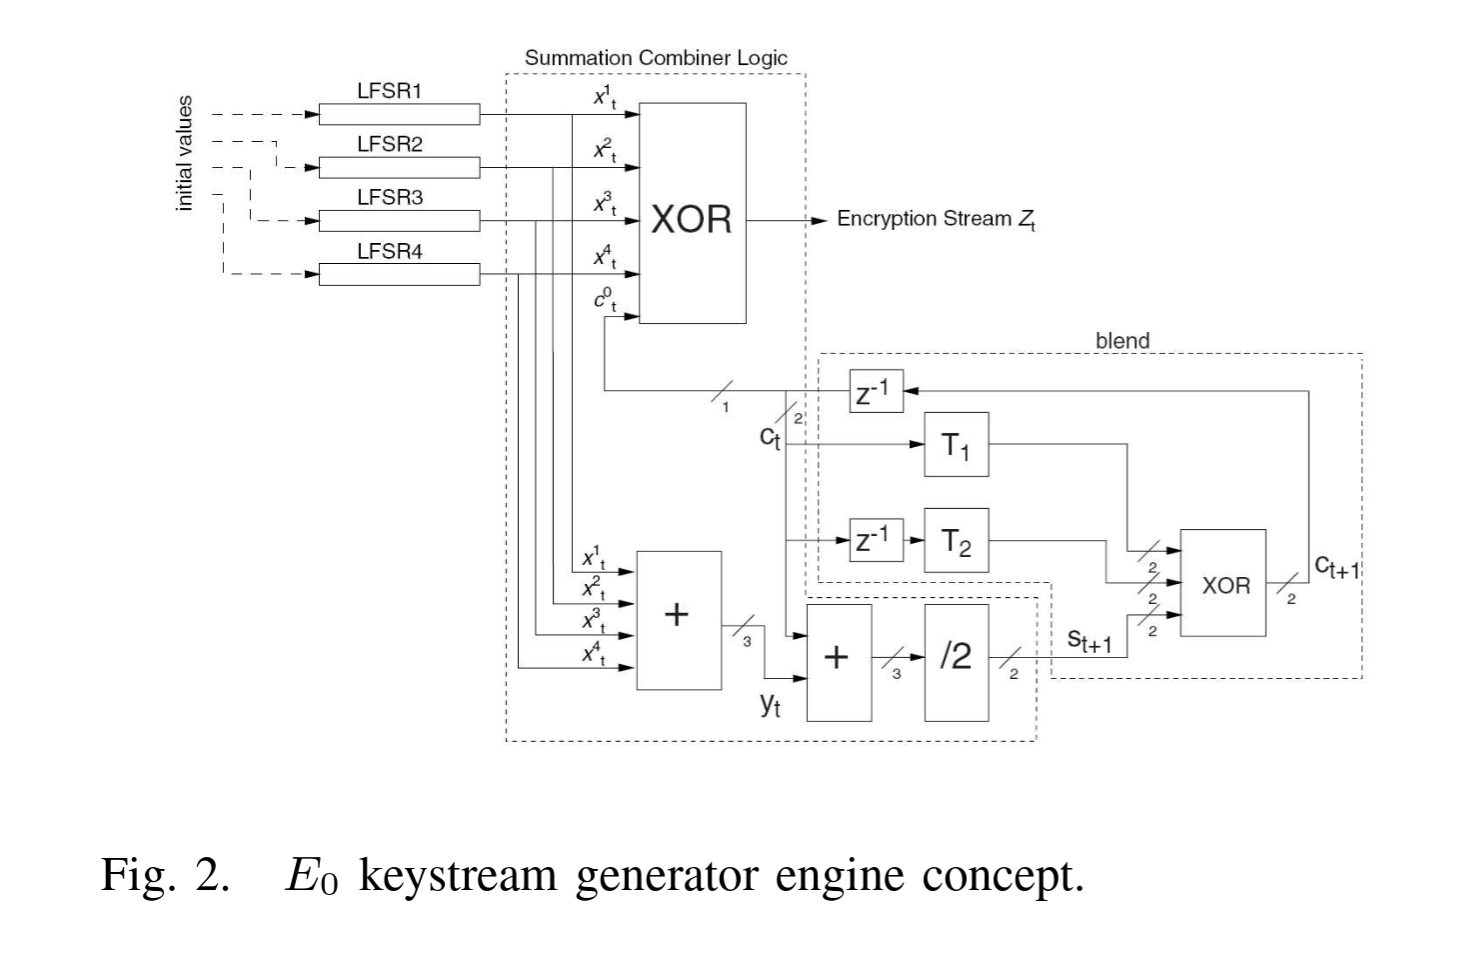
\includegraphics[width=0.75\textwidth]{image.png}
\end{figure}

Los bits del vector $\mathbf{x}_t$ no se usan directamente, sino que se introducen en una máquina de
estados finitos denominada \textit{Summation Combiner Logic and Blend} (SCLB). Esta máquina posee
4 bits de memoria organizados en el estado actual $\mathbf{c}_t = (c_t^1, c_t^0)$ y el estado anterior
$\mathbf{c}_{t-1} = (c_{t-1}^1, c_{t-1}^0)$.

El funcionamiento matemático del SCLB se define mediante las siguientes operaciones:

\textbf{1. Suma aritmética (El componente no lineal):} El sistema calcula la suma en los números
enteros (no en módulo 2) de las salidas de los registros:

\centerline{$y_t = \displaystyle\sum_{i=1}^{4} x_t^i$}

Como estamos sumando 4 bits, el resultado puede ser $y_t \in \{0, 1, 2, 3, 4\}$.

\textbf{2. Generación del bit de cifrado (Operación lineal en $\mathbb{F}_2$):} El bit de salida $z_t$, que
formará parte del \textit{keystream} definitivo, se calcula mediante la suma módulo 2 (XOR) de
los bits de los registros y el bit menos significativo del estado actual:

\centerline{$z_t = x_t^1 \oplus x_t^2 \oplus x_t^3 \oplus x_t^4 \oplus c_t^0$}

\textbf{3. Actualización del estado (Mezcla y bijecciones lineales):} Para calcular el siguiente
estado, el sistema determina un valor intermedio $s_{t+1}$ que actúa como un acarreo
(\textit{carry}), basándose en la suma entera anterior:

\centerline{$s_{t+1} = \begin{bmatrix} s_{t+1}^0 & s_{t+1}^1 \end{bmatrix} = \left\lfloor \dfrac{y_t + c_t}{2} \right\rfloor \in \{0, 1, 2, 3\}$}

Finalmente, el nuevo estado $\mathbf{c}_{t+1}$ se obtiene aplicando transformaciones algebraicas:

\centerline{$\mathbf{c}_{t+1} = \begin{bmatrix} c_{t+1}^0 & c_{t+1}^1 \end{bmatrix} = s_{t+1} \oplus T_1[\mathbf{c}_t] \oplus T_2[\mathbf{c}_{t-1}]$}

Es fundamental destacar que $T_1$ y $T_2$ son bijecciones lineales sobre el campo de Galois
$\mathrm{GF}(4)$ (equivalente a nuestro espacio $\mathbb{F}_2^2$). Al ser transformaciones lineales, en la
implementación real se construyen mediante simples operaciones matriciales (puertas lógicas
XOR), conectando de nuevo este sistema criptográfico con los fundamentos del álgebra lineal.

\smalltitle{2.6.3. Criptoanálisis como un problema de sistemas de ecuaciones lineales}

El objetivo de un ataque criptográfico contra este sistema es recuperar el vector inicial de
128 bits. Investigaciones recientes demuestran que vulnerar esta seguridad se reduce a un
problema algebraico a gran escala.

Si un atacante logra interceptar el bit $z_t$, puede usar la ecuación de generación del bit de
cifrado para plantear hipótesis sobre el estado $c_t^0$. Aislando las incógnitas (los bits de
los registros), la ecuación queda expresada como una ecuación lineal booleana clásica:

\centerline{$x_t^1 \oplus x_t^2 \oplus x_t^3 \oplus x_t^4 = c_t^0 \oplus z_t$}

El ataque consiste en aplicar un proceso de iteración hacia atrás (\textit{backtracking}). Gracias a
que el valor intermedio $y_t$ depende solo de la suma entera y no del valor individual de cada
bit, el atacante puede descartar ramas enteras de posibilidades. A medida que avanza, va
recolectando ecuaciones lineales de la forma descrita arriba.

Cuando el atacante logra formar un sistema de 128 ecuaciones lineales booleanas linealmente
independientes, puede resolverlo utilizando matrices y operaciones de álgebra lineal estándar.
La solución a ese enorme sistema matricial revelará el vector inicial de los registros, rompiendo
por completo la clave secreta del Bluetooth.




\newpage
\bigtitle{3. Aplicación práctica}
\medtitle{3.1 Explicación sobre ejemplo práctico}
El ejemplo elegido es un envío de audio desde un teléfono móvil a unos auriculares compatibles
por Bluetooth.

En primer lugar, el audio se digitaliza y se representa como una secuencia de datos binarios que
puede interpretarse como un vector perteneciente a un espacio vectorial. Este vector se somete a
una codificación en la que se introduce redundancia mediante matrices generadoras para detectar
y corregir errores (ya sean externos o internos a la comunicación entre los dos dispositivos).

Tras este proceso, los datos previamente codificados se transforman en señales físicas mediante
procesos de modulación similares a transformaciones lineales entre espacios vectoriales. Además,
al estar estas señales conectadas a través de un canal inalámbrico, se deben tener en cuenta las
perturbaciones causadas por el ruido y las interferencias que puedan ocurrir.

Posteriormente, el receptor de la señal, es decir los auriculares, aplica técnicas algebraicas para
estimular el mensaje original a partir de la señal recibida. Estas técnicas permiten identificar si el
vector recibido pertenece al subespacio de señales válidas. Si no es así, permiten aproximarlo al
vector válido más cercano.

Finalmente, se recupera el mensaje inicialmente enviado para que el usuario perciba la señal sin
interrupciones considerables.



A continuación, realizaremos una demostración similar a la del ejemplo explicado en este punto,
demostrándolo matemáticamente paso a paso.






\newpage
\medtitle{3.2 Ejemplo práctico paso a paso}
Suponiendo que un dispositivo envía este vector como mensaje binario (teniendo en cuenta
que pertenece a $\mathbb{F}_2^2$):\\
                                  \centerline{$m = (1,0)$}

\smalltitle{3.2.1 Codificación del vector mediante matrices generadoras}
Sea la matriz generadora:

\centerline{$G = \begin{pmatrix}1 & 0 \\ 0 & 1 \\ 1 & 1\end{pmatrix}\in\mathbb{F}_2^{3\times 2}$}

Realizando el producto matricial:

\[
c=Gm=\begin{pmatrix}1 & 0 \\ 0 & 1 \\ 1 & 1\end{pmatrix}
\begin{pmatrix}1 \\ 0\end{pmatrix}
=
\begin{pmatrix}1 \\ 0 \\ 1\end{pmatrix}
\]



Por tanto, el vector codificado es:

\centerline{$c = \begin{pmatrix}1 \\ 0 \\ 1\end{pmatrix}$}

Este vector pertenece a un subespacio vectorial de $\mathbb{F}_2^3$, generado por las columnas de la
matriz G. Dicho subespacio es la base para la detección y corrección de errores de esta
comunicación.

\smalltitle{3.2.2 Modelización de la señal transmitida}
Una vez codificada la información, esta debe transformarse en una señal física. Este
proceso (modulación) puede modelizarse como una transformación lineal en un espacio
vectorial continuo.

Si se consideran n muestras de la señal transmitida, esta puede representarse como un
vector:

\centerline{$s=(s_1,s_2,s_3)\in\mathbb{R}^3$}

En este caso, se adopta un modelo simplificado en el que la modulación viene dada por una
matriz identidad:

\centerline{$s=Mc,\; M=I$}


\newpage
Por tanto:



\centerline{$s = \begin{pmatrix}1 \\ 0 \\ 1\end{pmatrix}$}



\smalltitle{3.2.3 Modelización del canal de transmisión}
Durante la transmisión, la señal atraviesa un canal inalámbrico que introduce alteraciones
debido a interferencias, ruido y otros fenómenos físicos. Este proceso puede modelizarse
mediante la ecuación:

\centerline{$r = Hs + n$}

Donde:

$H\in\mathbb{R}^{3\times 3}$ es la matriz del canal,

$s$ es la señal transmitida,

$n$ es un vector de ruido,

$r$ es la señal recibida.

En este ejemplo, se considera un canal sin distorsión estructural, por lo que:

\centerline{$H=I$}

Sin embargo, se introduce un vector de ruido:

\centerline{$n = \begin{pmatrix}0 \\ 1 \\ 0\end{pmatrix}$}



Por lo tanto, la señal recibida es:

\[
r = \begin{pmatrix}1 \\ 0 \\ 1\end{pmatrix}
+ \begin{pmatrix}0 \\ 1 \\ 0\end{pmatrix}
= \begin{pmatrix}1 \\ 1 \\ 1\end{pmatrix}
\]

Este resultado refleja la señal alterada debido al ruido anteriormente mencionado del canal.
\newpage
\smalltitle{3.2.4 Detección de errores mediante distancia de Hamming}
Para analizar las diferencias entre la señal transmitida y la recibida, se emplea distancia de
Hamming (mencionado en 2.1.3).

Sean:
$c = \begin{pmatrix}1 \\ 0 \\ 1\end{pmatrix},\quad r = \begin{pmatrix}1 \\ 1 \\ 1\end{pmatrix}$

La distancia de Hamming viene dada por: $d_H(c,r)=1$.

Se puede observar a simple vista que este resultado indica que se ha producido un error en
una de las posiciones del vector transmitido. Además, esta distancia permite cuantificar la
proximidad entre vectores en el espacio discreto, lo cual es útil para la detección de errores.

\smalltitle{3.2.5 Detección mediante matriz de control}
Además de la distancia de Hamming, los códigos lineales ayudan a detectar errores
mediante matrices de control de paridad. Sea la matriz:

\centerline{$H=\begin{pmatrix}1&1&1\end{pmatrix}$}

Para que un vector c sea válido, debe cumplirse:

\centerline{$Hc = 0$}

Sin embargo, al recibir r, se calcula:





\centerline{$Hr=\begin{pmatrix}1&1&1\end{pmatrix}\begin{pmatrix}1 \\ 1 \\ 1\end{pmatrix}=3\equiv 1\;(\mathrm{mod}\;2)$}

Dado que: $Hr\neq 0$, se concluye que el vector recibido no pertenece al subespacio de códigos válidos, es decir,
se confirma la presencia de un error.
\newpage
\smalltitle{3.2.6 Correción mediante proyección en subespacios}
El conjunto de palabras válidas del código forma un subespacio vectorial $W\subseteq\mathbb{F}_2^3$. La señal
recibida r puede no pertenecer al subespacio debido al ruido, por lo tanto, ahora se debe
encontrar el vector $c\in W$ más cercano a $r$.

En este caso, los vectores válidos son:
$\begin{pmatrix}0 \\ 0 \\ 0\end{pmatrix},\quad \begin{pmatrix}1 \\ 0 \\ 1\end{pmatrix},\quad \begin{pmatrix}0 \\ 1 \\ 1\end{pmatrix},\quad \begin{pmatrix}1 \\ 1 \\ 0\end{pmatrix}$
Se calcula la distancia de Hamming entre r y cada uno de ellos, obteniendo que el vector
más cercano es:

\centerline{$\hat{c}=\begin{pmatrix}1 \\ 0 \\ 1\end{pmatrix}$}

\smalltitle{3.2.7 Recuperación del mensaje original}

Finalmente, una vez obtenido el vector corregido c, se procede a recuperar el mensaje
orginal m. Dado que:

\centerline{$c=Gm$}

Y que ya se conoce la matriz generadora, se puede determinar definitivamente que:

\centerline{$m = \begin{pmatrix}1 \\ 0\end{pmatrix}$}

El resultado coincide con el mensaje inicial, por lo tanto, se puede confirmar que el proceso
el proceso de codificación y correción de errores descrito en este apartado es correcto.





\newpage
\bigtitle{4. Conclusión}
\newpage
\bigtitle{5. Referencias}
IACR ePrint Archive. (2022). An algebraic attack to the Bluetooth stream cipher E0 (Report 2022/016). \url{https://eprint.iacr.org/2022/016.pdf}

The confidentiality - integrity - accessibility triad into the knowledge security: A reassessment from the point of view of the knowledge contribution to innovation. (n.d.). ResearchGate. \url{https://www.researchgate.net/publication/257985911_The_Confidentiality_-_Integrity_-_Accessibility_Triad_into_the_Knowledge_Security_A_Reassessment_from_the_Point_of_View_of_the_Knowledge_Contribution_to_Innovation}

Gallager, R. G. (2008). Principles of digital communication. Cambridge University Press.

Lay, D. C. (2012). Linear algebra and its applications. Pearson.

Lin, S., \& Costello, D. J. (2004). Error control coding. Pearson.

Oppenheim, A. V., \& Schafer, R. W. (2010). Signals and systems (2nd ed.). Prentice Hall.

Haykin, S. (2002). Adaptive filter theory (4th ed.). Prentice Hall.

ScienceDirect. (n.d.). Parity-check matrix. \url{https://www.sciencedirect.com/topics/computer-science/parity-check-matrix}

Nota: Se ha usado IA (ChatGPT/Gemini) para correcciones ortográficas, organización del documento y proofreading.




\newpage
\endgroup
\end{document}
